\documentclass[border=1mm]{standalone}
\usepackage{tikz,tkz-euclide}
\usepackage{pgfplots}
\usetikzlibrary{arrows,calc,patterns,intersections}
\begin{document}

%\begin{tikzpicture}
%
%\tikzset{
%    dot/.style={circle,inner sep=1pt,fill,label={\tiny #1},name=#1}}
%    
%    
%\node[dot=A] (A) at (0,0) {};
%\node[dot=B] (B) at (1,0) {};
%\node[dot=C] (C) at (0,1) {};
%\node[dot=D] (D) at (1,0.5) {};
%
%\draw [name path=A--B] (A) -- (B);
%\draw [name path=C--D] (C) -- (D);
%
%\coordinate (E) at (intersection of A--B and C--D);
%\node[dot=E]  at (E) {};
%\draw[dotted] (B)--(E)--(D);
%\end{tikzpicture}


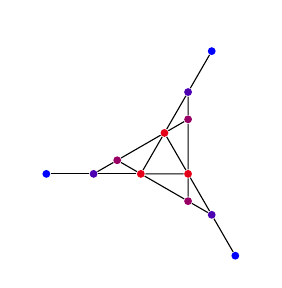
\begin{tikzpicture}[scale=0.6]

\tikzset{
    dot/.style={circle,inner sep=1pt,fill,label={\tiny #1},name=#1}}

\node at (-2.2,0) {~};    
\node at (2.2,0) {~};    
    
\node[dot, fill=blue!10!red] (A) at (0,0) {};
\node[dot, fill=blue!10!red] (B) at (1,0) {};
\node[dot, fill=blue!10!red] (C) at (0.5,{0.5*sqrt(3)}) {};
\node[dot, fill=blue!70!red] (D) at (-1,0) {};
\node[dot, fill=blue!100!red] (E) at (-2,0) {};
\node[dot, fill=blue!70!red] (F) at (1.5,{-0.5*sqrt(3)}) {};
\node[dot, fill=blue!100!red] (G) at (2,{-1*sqrt(3)}) {};
\node[dot, fill=blue!70!red] (H) at (1,{1*sqrt(3)}) {};
\node[dot, fill=blue!100!red] (I) at (1.5,{1.5*sqrt(3)}) {};

\draw [name path=A--F, draw=none] (A) -- (F);
\draw [name path=B--H, draw=none] (B) -- (H);
\draw [name path=C--D, draw=none] (C) -- (D);

\coordinate (X) at (intersection of A--F and B--H);
\node[dot, fill=blue!40!red] (X1) at (X) {};

\coordinate (Y) at (intersection of A--F and C--D);
\node[dot, fill=blue!40!red] (Y1) at (Y) {};

\coordinate (Z) at (intersection of B--H and C--D);
\node[dot, fill=blue!40!red] (Z1) at (Z) {};


\draw (A) -- (B) -- (C) -- (A);
\draw (A) -- (D) -- (E);
\draw (B) -- (F) -- (G);
\draw (C) -- (H) -- (I);

\draw (X1) -- (B) -- (Z1) -- (H);
\draw (Y1) -- (A) -- (X1) -- (F);
\draw (Z1) -- (C) -- (Y1) -- (D);

\end{tikzpicture}

\end{document}
